\documentclass{csse4400}

% \teachermodetrue

\usepackage{float}

\usepackage{languages}

\title{Events \& Worker Queues}
\author{Evan Hughes \& Brae Webb}

\date{\week[practical]{7}}
\begin{document}

\maketitle

\begin{figure}[ht]
    \centering
    
\includegraphics[width=0.8\textwidth]{images/event-driven}
\end{figure}

\section{This Week}
Our goal is to:
\begin{itemize}
    \item Explore events and worker queues in the context of AWS.
    \item Deploy our own TaskOverflow container on AWS Elastic Container Registry (ECS).
    \item Develop an event-based architecture to generate a calendar from tasks in TaskOverflow.
\end{itemize}

\section{Event Processing}

As we saw in Event-Driven Architectures \cite{events-notes},
event processing enable us to build highly scalable and extensible systems.
In this practical we will get our hands dirty with event processing using AWS SQS.
AWS SQS is a service which acts as an event broker.

\subsection{Technologies}

There are other technologies that can be useful in developing an event-based architecture.
The following is a non-exhaustive list of services native to AWS.

\subsubsection{AWS SQS}

AWS provides the Simple Queue Service, SQS,
which offers a simple and fully managed message queue service.
There are two flavours of SQS to be aware of.
\begin{description}
    \item[Standard message queues] allow for greater scalability by providing higher through-put.
However, standard message queues in SQS are not exactly queues,
messages are not first in first out,
they are best-effort ordered.
    \item[FIFO message queues] guarantees that messages are First in First Out.
\end{description}

\subsubsection{AWS SNS}
\begin{quote}{AWS}
Amazon Simple Notification Service (Amazon SNS) is a fully managed messaging service for both application-to-application (A2A) and application-to-person (A2P) communication.

The A2A pub/sub functionality provides topics for high-throughput,
push-based, many-to-many messaging between distributed systems,
microservices, and event-driven serverless applications.
Using Amazon SNS topics,
your publisher systems can fanout messages to a large number of subscriber systems,
including Amazon SQS queues, AWS Lambda functions,
HTTPS endpoints, and Amazon Kinesis Data Firehose,
for parallel processing.
The A2P functionality enables you to send messages to users at scale via SMS, mobile push, and email.
\end{quote}

\subsubsection{AWS MQ / Apache ActiveMQ / RabbitMQ}
\begin{quote}{AWS}
Amazon MQ is a managed message broker service for Apache ActiveMQ and RabbitMQ that makes it easy to set up and operate message brokers on AWS.
Amazon MQ reduces your operational responsibilities by managing the provisioning, setup, and maintenance of message brokers for you.
Because Amazon MQ connects to your current applications with industry-standard APIs and protocols,
you can easily migrate to AWS without having to rewrite code.
\end{quote}

\aside{Not available in the lab environments}

\subsubsection{AWS MSK ( Managed Streaming for Apache Kafka )}
\begin{quote}{AWS}
Amazon Managed Streaming for Apache Kafka (Amazon MSK) is a fully managed service that enables you to build and run applications that use Apache Kafka to process streaming data.
Amazon MSK provides the control-plane operations, such as those for creating, updating, and deleting clusters.
It lets you use Apache Kafka data-plane operations,
such as those for producing and consuming data
It runs open-source versions of Apache Kafka.
This means existing applications, tooling, and plugins from partners and the Apache Kafka community are supported without requiring changes to application code.
You can use Amazon MSK to create clusters that use any of the Apache Kafka versions listed under Supported Apache Kafka versions.
\end{quote}

\aside{Not available in the lab environments}

\subsubsection{Redis}
\begin{quote}{AWS}
Redis, which stands for Remote Dictionary Server,
is a fast, open source, in-memory, key-value data store.
The project started when Salvatore Sanfilippo,
the original developer of Redis,
wanted to improve the scalability of his Italian startup.
From there, he developed Redis,
which is now used as a database, cache, message broker, and queue.

Redis delivers sub-millisecond response times,
enabling millions of requests per second for real-time applications in industries like gaming, ad-tech, financial services, healthcare, and IoT.
Today, Redis is one of the most popular open source engines today,
named the ``Most Loved'' database by Stack Overflow for five consecutive years.
Because of its fast performance,
Redis is a popular choice for caching, session management, gaming, leaderboards, real-time analytics, geospatial, ride-hailing, chat/messaging, media streaming, and pub/sub apps.
  
AWS offers two fully managed services to run Redis.
Amazon MemoryDB for Redis is a Redis-compatible, durable, in-memory database service that delivers ultra-fast performance.
Amazon ElastiCache for Redis is a fully managed caching service that accelerates data access from primary databases and data stores with microsecond latency.
Furthermore, ElastiCache also offers support for Memcached, another popular open source caching engine.
\end{quote}

\aside{Not available in the lab environments}

\section{Talking to the Simple Queue Service (SQS)}

\warning{
    For terminal examples in this section,
    lines that begin with a \$ indicate a line which you should type while the other lines are example output that you should expect.
    Not all of the output is captured in the examples to save on space.  
}

Today we will be creating and experimenting with the two queue flavours of AWS SQS.
A standard queue, named \texttt{csse6400\_prac} and a FIFO queue, named \texttt{csse6400\_prac.fifo}.
The Terraform code below can be used to create these two queues.

\info{
  If you have forgotten how to get started you will need to run the following commands in a local terminal.

  \bash{
    terraform init^^J
    ...^^J
    $ terraform plan^^J
    ...^^J
    $ terraform apply^^J
    ...
  }
}

\teacher{
  In the below terraform it is pretty simple and relies a lot on defaults.
  Though the FIFO name needs to have .fifo at the end, make sure to mention this.
}

\begin{code}[language=terraform, numbers=none]{}
terraform {
  required_providers {
    aws = {
      source = "hashicorp/aws"
      version = "~> 3.0"
    }
  }
}

provider "aws" {
  region = "us-east-1"
  shared_credentials_file = "./credentials"
}

resource "aws_sqs_queue" "our_first_mailbox" {
  name                        = "csse6400_prac"
}

resource "aws_sqs_queue" "our_first_fifo" {
  name                        = "csse6400_prac.fifo"
  fifo_queue                  = true
  content_based_deduplication = true
}

output "mailbox" {
  value = aws_sqs_queue.our_first_mailbox.arn
}

output "fifo" {
  value = aws_sqs_queue.our_first_fifo.arn
}
\end{code}

Now that we have provisioned the queues we can have a look at them in the AWS Console.
In the main AWS dashboard you can search for ``SQS'' to find these queues.
You should reach a page like this:

\begin{figure}[H]
  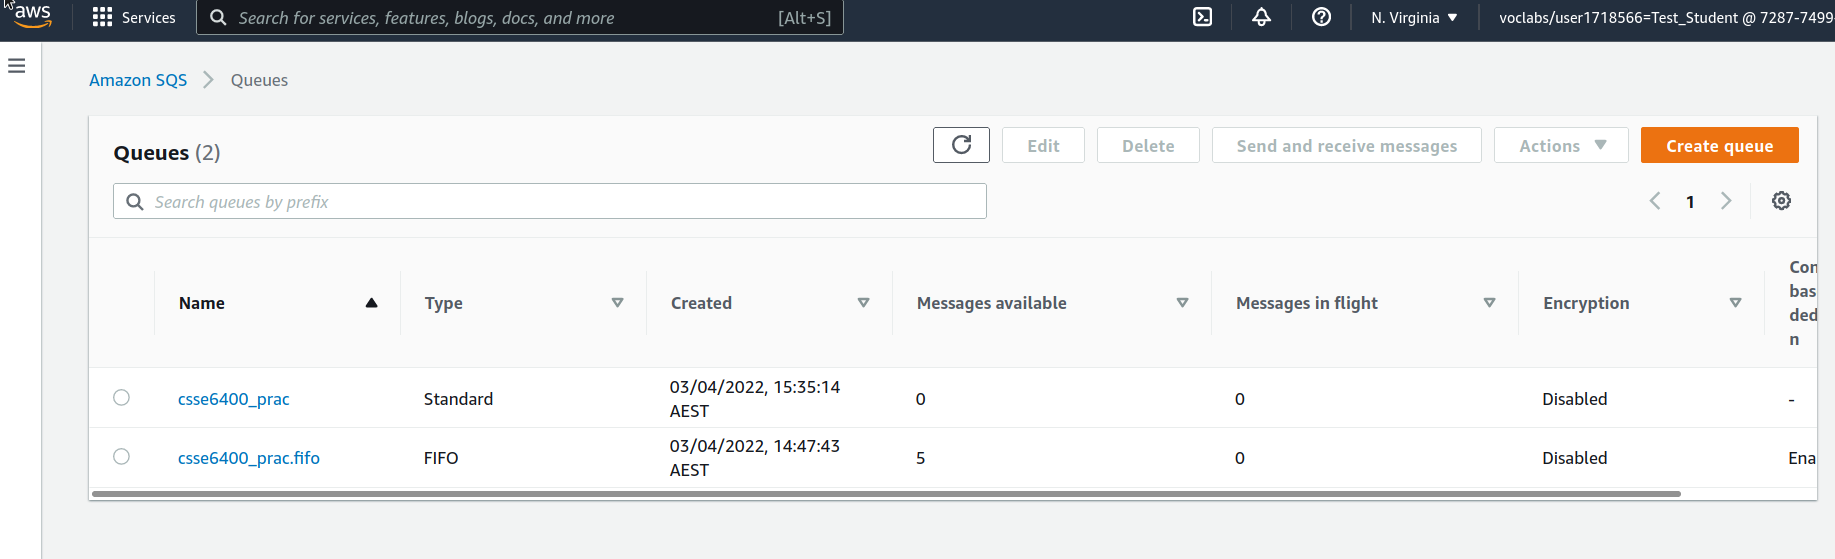
\includegraphics[width=\textwidth]{images/sqspanel}
\end{figure}

Like the EC2 and RDS dashboards,
we can browse the queue configurations and metrics.
  
\teacher{
  Show the students the Monitoring Panel and Access Policy panel in particular.

  \begin{itemize}
    \item Monitoring: Messages Sent/Received
    \item Monitoring: Empty Receives - This is the receiver getting nothing from polling. Costs \$ in the real world.
    \item Policy: Not covering today but SQS is a public service, it is protected via AWS credentials. In real use cases you need to configure a Access Policy.
  \end{itemize}
}

\subsection{Queue Command-line Interface}

We have provided a small docker container for you to use with your queues to see the differnce between the implementations.
First we must retrieve our AWS credentials and setup our environment.

With our learner lab grab the AWS credentials but instead of creating a credentials file we will be using environment variables.
Make a folder for the practi.

\begin{code}[language=shell, numbers=none]{}
$ mkdir queues && cd queues
\end{code}

Now we need to create an environment file for our docker container to read so that it can access AWS. Create a ``.env'' file in the current directory and edit the contents so that it looks similar to the below: The AWS keys will be from the credentials shown in your lab environment.

\begin{code}[numbers=none]{}
TERM=xterm-256color
AWS_ACCESS_KEY_ID=...
AWS_SECRET_ACCESS_KEY=...
AWS_SESSION_TOKEN=...
\end{code}

\begin{code}[numbers=none,keepspaces=true]{}
$ docker run --rm -it --env-file .env ghcr.io/csse6400/queue:main --name "test" --client-name "Client 1"


  __________
 |   \XX/   |
 | T. \/ .T |      University of Queensland
 | XX:  :XX |          Faculty of EAIT
 T L' /\ 'J T
  \  /XX\  /         CSSE6400 Queue Prac
@\_ '____' _/@       csse6400.uqcloud.net
\_X\_ __ _/X_/
 \=/\----/\=/



Unable to find a Queue by this name test
\end{code}

If your program shows the above then your ready to head to the next section :).
  

% \begin{code}[language=shell, numbers=none]{}
% docker run --rm -it --env-file .env ghcr.io/csse6400/queue:main --name "csse6400_prac" --client-name "hello" --sender
% \end{code}

% \begin{code}[language=shell, numbers=none]{}
%   docker run --rm -it --env-file .env ghcr.io/csse6400/queue:main --name "csse6400_prac" --client-name "hello" --sender
% \end{code}
  



\subsection{SQS Standard}

As we have stated above the ``Standard'' offering of SQS does not guarantee order or ``only once delivery''. 
Assuming our terraform was created sucessfully we are going to create one publisher and one subscriber.

\info{
  For the rest of this practical you will require multiple terminals. Make sure these are all in the same folder so we can reuse the .enf file. 
}

To create the subscriber run the following command:

\begin{code}[numbers=none,keepspaces=true]{}
  $ docker run --rm -it --env-file .env ghcr.io/csse6400/queue:main --name "csse6400_prac" --client-name "Client 1" --receive
\end{code}

\begin{figure}[H]
  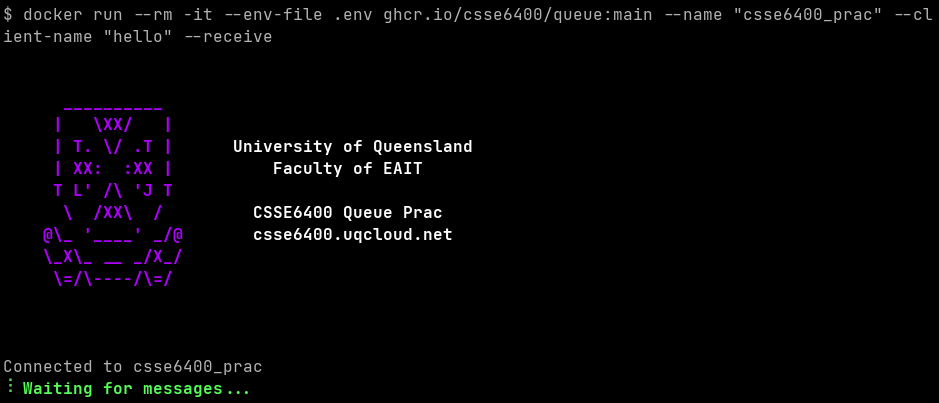
\includegraphics[width=\textwidth]{images/stacksub}
\end{figure}

Now lets start a publisher in another terminal but keep both terminals on your screen if you have space.

\begin{code}[numbers=none,keepspaces=true]{}
  $ docker run --rm -it --env-file .env ghcr.io/csse6400/queue:main --name "csse6400_prac" --client-name "Client 1"
\end{code}

\begin{figure}[H]
  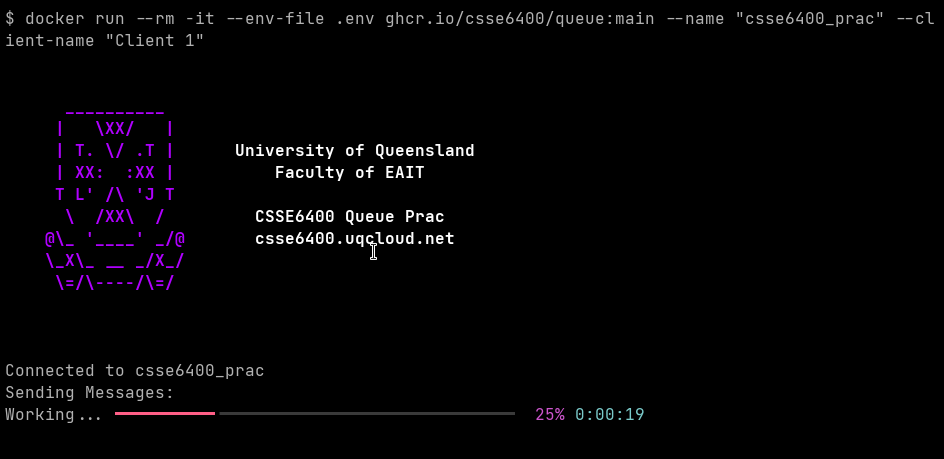
\includegraphics[width=\textwidth]{images/stackpub}
\end{figure}

When the publisher connects to the Queue it is going to put 100 messages of increasing increment into the queue. On the subscriber we will be able to see the messages being received, an example is provided below:

\begin{figure}[H]
  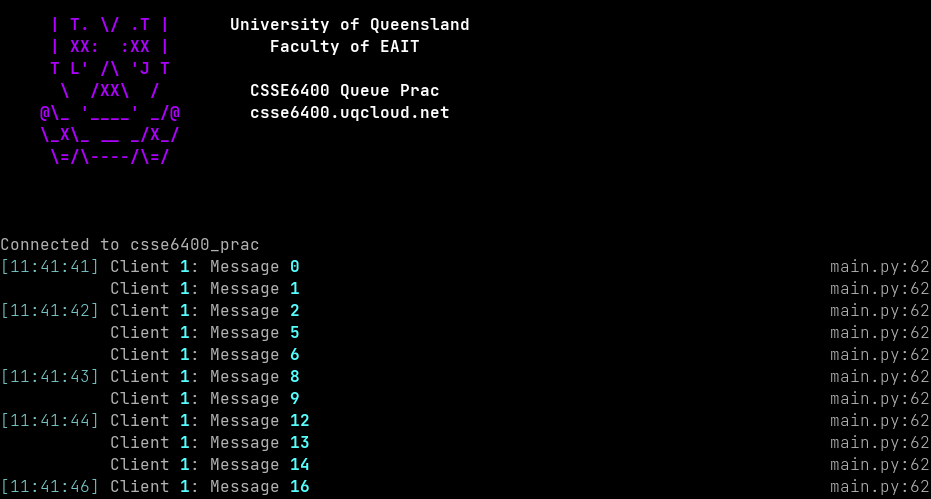
\includegraphics[width=\textwidth]{images/stacksubdata}
\end{figure}

hopefully like our example you can see that some of the messages arrive out of order. Next add more publishers and subscribers and experiment with the differnt configurations. 

\info{
  When making multiple publishes you may want to change the client-name cli parameter so you can keep track of when the messages arrived at the subscribers.
}


\subsection{SQS FIFO}
Now we will experiment with the FIFO based service offered by SQS. Like before we will start a subscriber but make sure the name of the queue matches the FIFO queue we created in terraform.

\begin{code}[numbers=none,keepspaces=true]{}
  $ docker run --rm -it --env-file .env ghcr.io/csse6400/queue:main --name "csse6400_prac.fifo" --client-name "Client 1" --receive
\end{code}

Now lets start a publisher in another terminal but keep both terminals on your screen if you have space.

\begin{code}[numbers=none,keepspaces=true]{}
  $ docker run --rm -it --env-file .env ghcr.io/csse6400/queue:main --name "csse6400_prac.fifo" --client-name "Client 1"
\end{code}

\begin{figure}[H]
  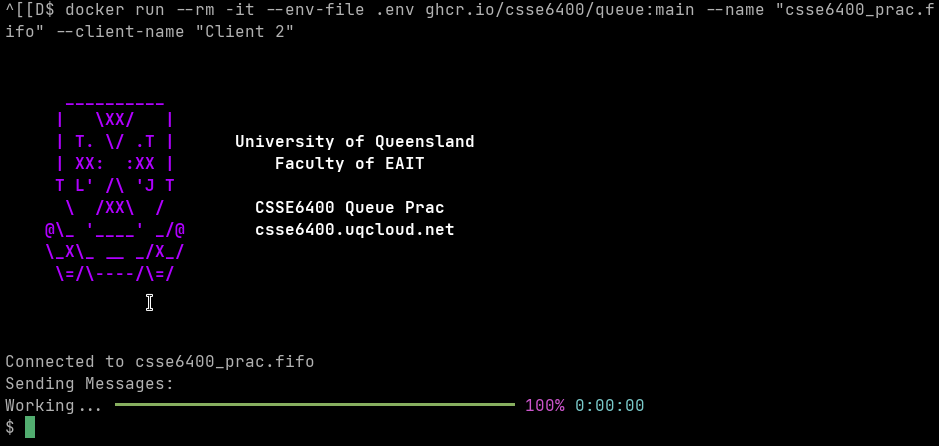
\includegraphics[width=\textwidth]{images/fifopub}
\end{figure}

On the subscriber we now see the messages arriving in order which is to be expected.

\begin{figure}[H]
  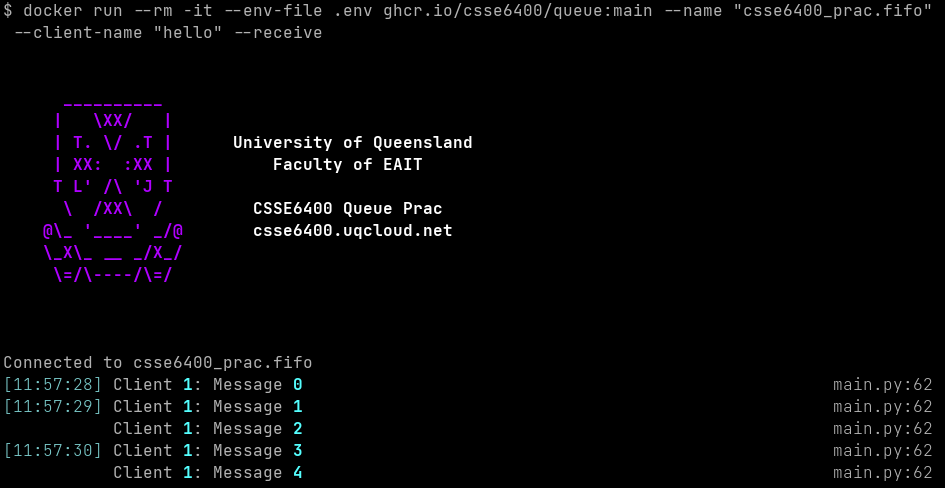
\includegraphics[width=\textwidth]{images/fifosub}
\end{figure}

If we re-run the publisher though we may not see any new messages make it to the consumer. This is because we have asked AWS to dedup messages where it can.

\teacher{
  Theres a cli param which prepends to the message to allow you to rerun if needed. It is --prepend "abcdef"
}

Again as before try experimenting with differnt publisher / subscriber configurations to see how they behave.

\info{
  When making multiple publishes you may want to change the client-name cli parameter so you can keep track of when the messages arrived at the subscribers.
}

\warning{
  \textbf{Please remember to terraform destroy to delete your resources}
}

\section{Hosting TaskOverflow Images}

When we last deployed a container on AWS,
we used an existing hosted image.
Now, we will be developing our own image so we will need a mechanism to host the image.
For this, we will being using a AWS ECR, Docker, and Terraform.
AWS ECR is the Elastic Container Registry,
it is a container registry like DockerHub or GitHub.
We can use it to host our images,
using the process below:

\begin{enumerate}
    \item Use Terraform to create an ECR repository for our image.
    \item Use Terraform to build our Docker image.
    \item Use Terraform to push our Docker image.
\end{enumerate}

\info{
This is a non-standard way process.
As you may have seen in the DevOps tutorial,
we would ordinarily like our code commits to trigger a CI/CD pipeline which builds appropriate images and pushes from there.
You can still use GitHub actions to build and push your container to the GitHub container registry and authenticate when you pull the image.

However, using ECR simplifies the process,
despite the oddities introduced by having a non-persistent ECR repository.
}

First we will setup our initial Terraform configuration.
Note that now we introduce a new required provider.
This provider is for Docker.

\begin{code}[language=terraform,numbers=none]{main.tf}
terraform {
   required_providers {
      aws = {
         source = "hashicorp/aws"
         version = "~> 4.0"
      }
      docker = {
         source  = "kreuzwerker/docker"
         version = "3.0.2"
      }
   }
}

provider "aws" {
   region = "us-east-1"
   shared_credentials_files = ["./credentials"]
}
\end{code}

As with our AWS provider,
when we initially configure the provider,
we want to authenticate so that we can later push to our registry using the Docker provider.
We will use the \texttt{aws\_ecr\_authorization\_token} data block to get appropriate ECR credentials for Docker.

\begin{code}[language=terraform,numbers=none]{main.tf}
data "aws_ecr_authorization_token" "ecr_token" {}

provider "docker" {
  registry_auth {
    address  = data.aws_ecr_authorization_token.ecr_token.proxy_endpoint
    username = data.aws_ecr_authorization_token.ecr_token.user_name
    password = data.aws_ecr_authorization_token.ecr_token.password
  }
}
\end{code}

We need to use Terraform to create an ECR repository to push to.

\begin{code}[language=terraform,numbers=none]{main.tf}
resource "aws_ecr_repository" "taskoverflow" {
  name = "taskoverflow"
}
\end{code}

The URL for containers in the ECR following the format below:

\url{{ACCOUNT_ID}.dkr.ecr.{REGION}.amazonaws.com/{REPOSITORY_NAME}}

Remember to push to a container registry,
we need a local container whose tag matches the remote URL.
We could then create and push the contianer locally with:

\begin{code}[language=bash,numbers=none]{}
docker build -t {ACCOUNT_ID}.dkr.ecr.{REGION}.amazonaws.com/{REPOSITORY_NAME} .
docker push {ACCOUNT_ID}.dkr.ecr.{REGION}.amazonaws.com/{REPOSITORY_NAME} 
\end{code}

However, it would be easier if we could build and push this container from within Terraform.
We can use the Docker provider for this.

\begin{code}[language=terraform,numbers=none]{image.tf}
resource "docker_image" "taskoverflow" {
  name         = "${aws_ecr_repository.taskoverflow.repository_url}:latest"
  build {
    context = "."
  }
}

resource "docker_registry_image" "taskoverflow" {
  name          = docker_image.taskoverflow.name
}
\end{code}

Notice that we are able to utilize the output of the ECR repository as the URL which resolves to the correct URL for the image.

\section{Worker Queues}

One good use case for queues is for distributing work to scale to demand.
In this exercise we encourage you to have a look at these widly used libraries to see how you could integrate them into a distributed system.

\begin{itemize}
  \item Python: \href{https://docs.celeryq.dev/en/stable/}{Celery}
  \item Java: \href{https://www.rabbitmq.com/tutorials/tutorial-one-java.html}{RabbitMQ}
\end{itemize}

The two above libraries are integrated into many popular application frameworks.
Today we will be using the Python library Celery to create a simple worker queue for TaskOverflow.

\subsection{Celery}

Celery is a Python library which allows you to create a worker queue.
It is popular and used in many large scale applications.
It is also relatively easy to use and has comprehensive documentation.


\subsection{TaskOverflow}

TaskOverflow will use celery to distribute the work of generating a calendar view of tasks,
as this could be a time-intensive task.
This will be done by a worker which will run in a separate container.
The TaskOverflow server will place job requests on the Celery queue.
The worker will pick-up jobs and generate the calendar view.
The webserver can then display the calendar view to the user.

Calendar generation occurs asynchronously with this architecture.
The user will not have to wait for the calendar view to be generated and the webserver can handle other requests.

\todo{Add diagram}
\todo{Add worker cli startup option}
\todo{Add celery}
\todo{Add job request}

\subsubsection{Design Challenge}

Say we observe a user pattern that the majority of users will mark off multiple todo items at once. We have also moved our calendar from a PDF being displayed to the user to an iCal so that its visible in their chosen calendar application.

How could we improve the efficiency of our system to reduce the amount of time it takes to generate the calendar view?

\bibliographystyle{ieeetr}
\bibliography{books,ours}

\end{document}
